\documentclass[9pt]{beamer}
\usetheme{metropolis}
%\usetheme{Madrid}
\usepackage{mathtools}
\usepackage{bm}
\usepackage{esvect}
\usepackage{amsmath}
\usepackage{physics}
\usepackage{empheq}
\usepackage[many]{tcolorbox}
\input{pool/NextDefs.tex}

%$\vv{\bm{L}}

\title{A Conceptual Design for NEXT-HD}
 
%\subtitle{Basic concepts}
 
\author{JJ, JVM, FM, VH}
 
\institute{Donostia International Physics Center (DIPC)} % (optional)
 
%\date[October 6th, 2018] % (optional)
%{PHYSIS, SAN SEBASTIAN: 2-6 OCTOBER 2018}
 
%\logo{\includegraphics[height=0.5cm]{dipc.png}
%\includegraphics[height=0.5cm]{IB.png}}


\tcbset{highlight math style={enhanced,
  colframe=red!60!black,colback=yellow!50!white,arc=4pt,boxrule=1pt,
  }}

\newtcbox{\mybox}[1][]{nobeforeafter,math upper,tcbox raise base,
  enhanced,frame hidden,boxrule=0pt,interior style={top color=green!10!white,
  bottom color=green!10!white,middle color=green!50!yellow},
  fuzzy halo=1pt with green,drop large lifted shadow,#1}
\begin{document}

\frame{\titlepage}
\begin{frame}
\frametitle{NEXT-HD based in SiPMs}

\begin{columns}
\column{0.45\textwidth}

\blt\ An upgrade of the NEXT technology to the ton scale, based in replacing PMTs with SiPMs was proposed in 2017. The proposed detector was symmetric, with two identical sensor planes behind the transparent anodes. The sensor planes alternated large SiPMs or energy measurements, with small SiPMs for tracking measurements. 

 \column{0.45\textwidth}
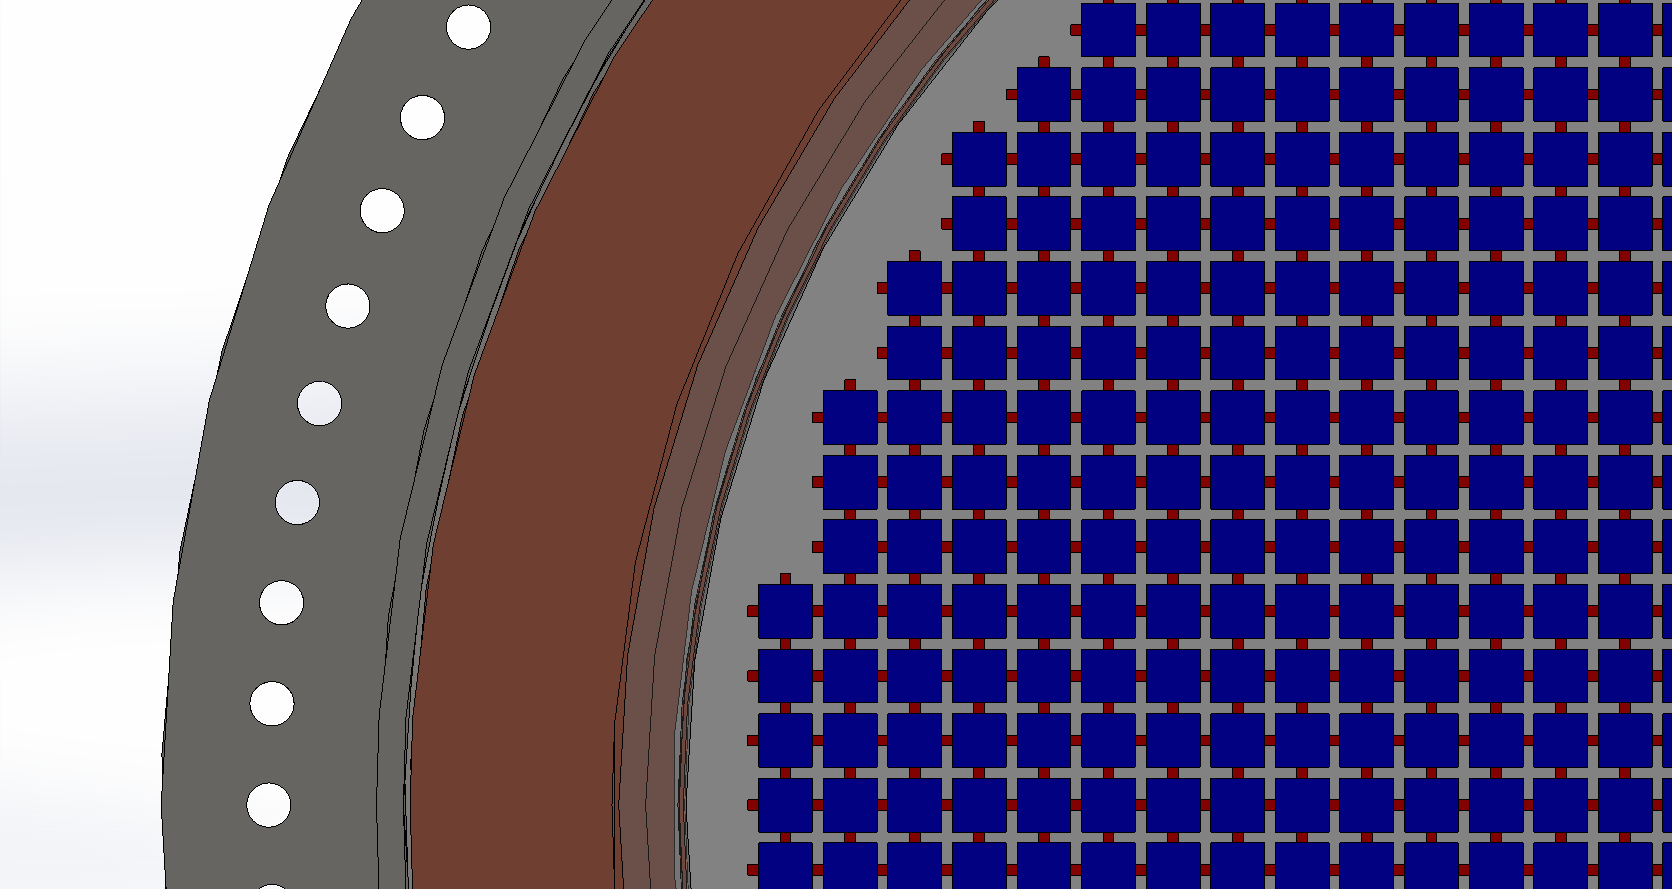
\includegraphics[scale=0.13]{img/n2-sector.png}

\end{columns}

\vspace{1cm}
{\fontsize{6pt}{7.2}\selectfont \bf Status of NEXT and prospects for a future Next Array apparatUS with Improved CApAbilities (NAUSICAA), J.J.  Gomez-Cadenas, PoS NEUTEL2017 (2018) 032.}
\end{frame}

\begin{frame}
\frametitle{NEXT-HD based in SiPMs: principle of operation}

\blt\ The small SiPMs (called tracking SiPMs or tSiPM) in each anode would perform the tracking function in the same way that currently done in \New\ and \Next.

\blt\ The large SiPMs (called energy SiPMs or eSiPM) in the opposite anode would perform the energy function, replacing the PMTs in \New\ and \Next.

\blt\ The eSiPMs of both planes would measure the primary scintillation needed for \tz.

\blt\ It was clear since the beginning that cool gas was necessary (FM, LA) to reduce DCR to manageable levels. 
\end{frame}

\begin{frame}
\frametitle{NEXT-HD based in SiPMs: size of SiPMs}

\blt\ The size of the tSiPMs can be chosen to be $\sim$\SI{1 x 1}{mm^2}, like  in \New\ and \Next.

\blt\ The eSiPMs must be chosen, a priory, as large as possible, to reduce the number of electronic channels. Choosing the eSiPMs size as \SI{10 x 10}{mm^2} results in \num{883572} channels (for a $\sim$ 90\% coverage). 

\blt\ Smaller SiPMs result in a very large number of channels (e.g, almost 3 M channels for \SI{3 x 3}{mm^2}). Reducing coverage results in reduced detection efficiency. 

\blt\ It was clear since the beginning that cool gas was necessary (FM, LA) to reduce DCR to manageable levels. 
\end{frame}

\begin{frame}
\frametitle{NEXT-HD based in SiPMs: \sone\ detection efficiency}

\blt\ The geometrical efficiency for the symmetric version of HD with SiPMs was computed by JMV to be 31.4 \%. Assuming a 40\% PDE for the SiPMs, the detection efficiency is 12.4 \%. 

\blt\ The number of scintillation photons produced by krypton deposits (assuming 
$W_s = 39.20$eV) is \num{1.06e+03}. Multiplying by the detection efficiency, one finds a total of \num{1.31e+02} detected photons from krypton. This implies an average
of \num{1.49e-04} photoelectrons per SiPM, a very small number. 

\blt\ The number of scintillation photons produced at \Qbb\ is \num{1.12e+05}. Multiplying by the detection efficiency, one finds a total of \num{7.78e+03} detected photons from krypton. This implies an average
of \num{8.80e-03} photoelectrons per SiPM, still a small number. 

\end{frame}

\begin{frame}
\frametitle{NEXT-HD based in SiPMs:  SiPM response}

\begin{columns}
\column{0.45\textwidth}

\blt\ Large SiPMs have large capacitance. A SiPM of \SI{10 x 10}{mm^2} has a capacitance of \SI{10}{ns}. As a consequence, the output waveform when connected to a readout will have a very long decay time, of the order of \SI{5}{\micro\second}.

\blt\ This implies that the output of the fast \sone\ signal will be a waveform which needs to be integrated up to \SI{5}{\micro\second}

 \column{0.45\textwidth}
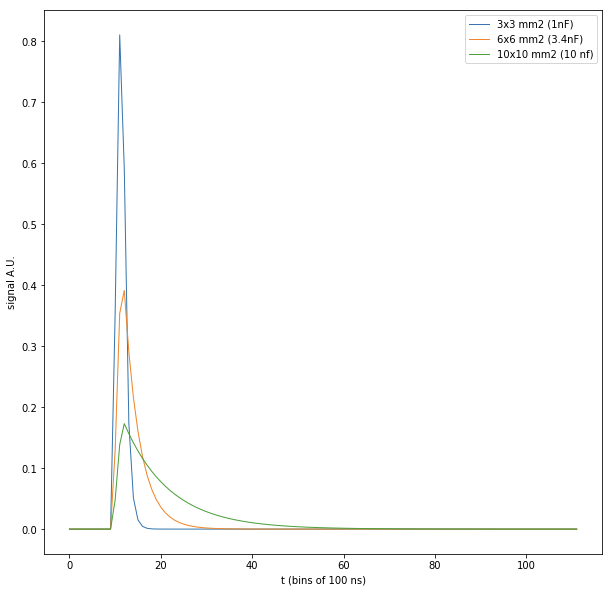
\includegraphics[scale=0.23]{img/sipmResponse.png}

\end{columns}
\end{frame}

\begin{frame}
\frametitle{NEXT-HD based in SiPMs:  DCR}

\begin{columns}
\column{0.45\textwidth}

\blt\ The dark current rate (DCR) of SiPMs is of the order of \SI{100}{\kilo\hertz\per\mm^2}, but decreases rapidly with temperature. 

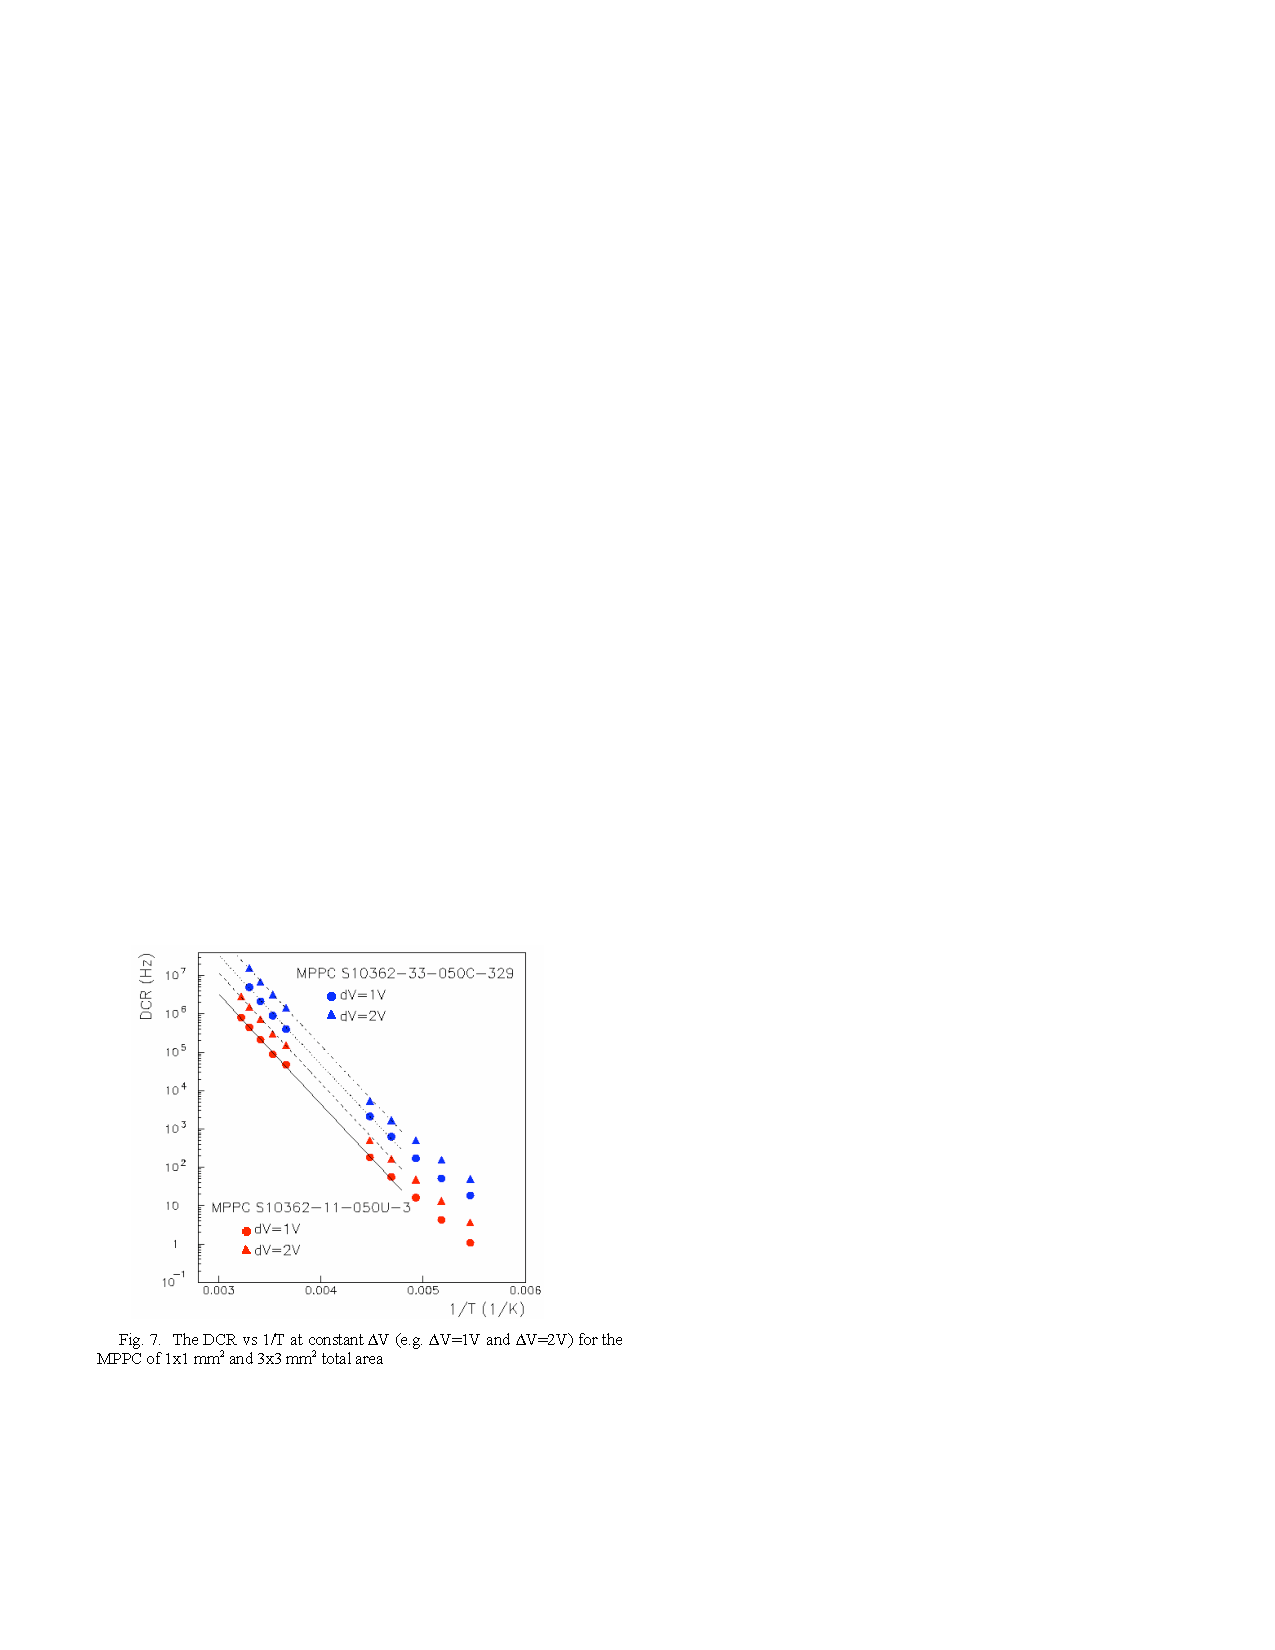
\includegraphics[scale=0.63]{img/dcR_T.pdf}

 \column{0.45\textwidth}
 
 \blt\ Unfortunately the noise per SiPM of \SI{10 x 10}{mm^2} in \SI{5}{\micro\second} is always larger than the \sone\ signal expected per SiPM at \Qbb

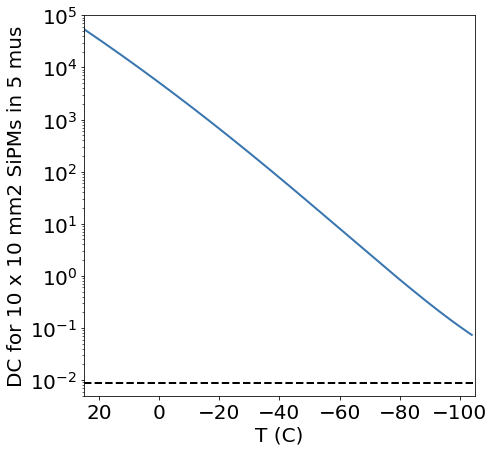
\includegraphics[scale=0.3]{img/dcr5mus.png}

\end{columns}

\blt Measuring \tz\ with a detector based in SiPMs is very difficult. 
\end{frame}



\begin{frame}
\frametitle{The Barrel and the Wheel}

\blt\ The idea of measuring \sone\ and/or \stwo\ using a WLS was proposed by DN many years ago. He suggested to possibilities. A barrel and a wheel. The barrel would run along the field cage, while the wheel could be place in the anode. In both cases, the detector would be a WLS plastic coated with another WLS, such as TPB or TPH. The role o the TPB (TPH) would be to shift impinging VUV light to blue light, that would then be capture by the barrel or the wheel and propagate by total internal reflection (TIR) to readout. 

\blt\ The problem with this implementation is that TPB (TPH) has the same refraction index that poly ($\sim 1.6$), and thus the light would end up propagating in the interface between TPB and xenon (which has much lower refraction index, $\sim 1$). But, since such a surface is very inhomogeneous, transmittance vanished quickly.
\end{frame}

\begin{frame}
\frametitle{Crying WOLF}

\blt\ A solution to this problem (JJGC, JMV, FM) is using Wavelength sifter OpticaL Fibres (WOLFs), which include one (or two) claddings ($n \sim 1.49$) which prevent light from reaching the TPB surface. Transmission is then restored. 

\blt\ Further advantages of WOLFs w.r.t. other solutions (such as the ARAPUCA designs, for DUNE) are robustness, availability (they are produce by two large manufacturers, Kuraray and St. Gobain) and cost.  

\blt\ In this way, both the Barrel and the Wheel (or rather the Wall) detectors can be resurrected. We call them BFD (Barrel Fibre detector) and AFD (Anode Fibre detector).  

\end{frame}

\begin{frame}
\frametitle{Principle of operation}
\begin{columns}
\column{0.45\textwidth}

\blt\ The basic component is a wavelength-shifting (WLS) optical fibre coated with TPB or another suitable VUV$\rightarrow$Blue WLS. The fibre itself is made of a polystyrene core ($n=1.6$) and an acrylic (double) cladding ($n=1.49$).

\blt VUV impinging upon the fibre is shifted to blue and enters the fibre where is eventually shifted to green and propagates by total internal reflection.
\column{0.45\textwidth}
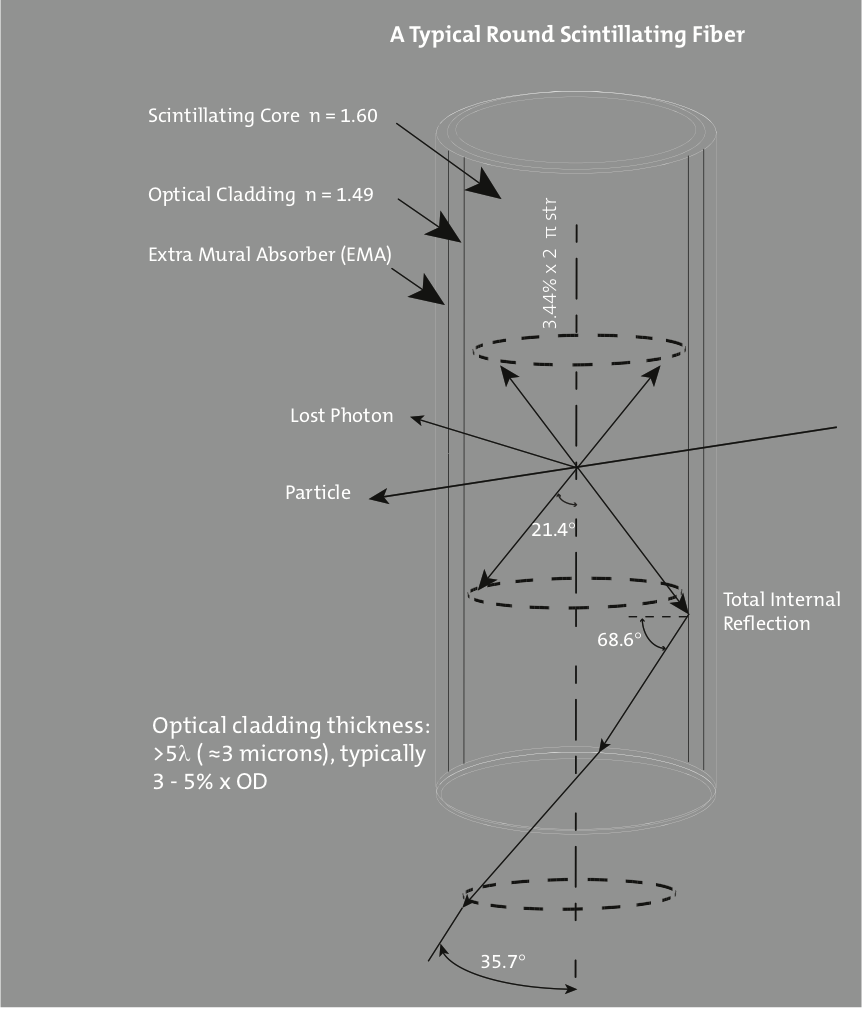
\includegraphics[scale=0.6]{img/fibers_tirf.png}

\end{columns}

\end{frame}


%\begin{frame}
%\frametitle{What is a field?}
%
%\begin{tcolorbox}[colback=white,arc=0pt,outer arc=0pt,colframe=black,boxrule=0.6pt]
%  \begin{center}
%    A field is a {\em device} that operates over a position in spacetime, $x^{\mu}$~ to produce an object representing the amplitude of something at that point in spacetime, $\phi(x^{\mu})$. The amplitude can be a {\em scalar}, a {\em vector}, a {\em complex number}, a {\em spinor} or a {\em tensor}. 
%
%  \end{center}
%\end{tcolorbox}
%
%\blt\ The concept of a field as an unseen entity which pervades space and time, connects with the concept of {\em ether}. 
%
%\blt\ Faraday grasped intuitively the idea of an electric or magnetic field that permeates all space and time. Maxwell codified Faraday?s idea and the electromagnetic field, together with all the paraphernalia of field theory, was born. 
%
%\blt\ In classical physics we understand that gravity is a field, electromagnetism is a field, and each can be described by a set of equations which governs their behavior. The field can oscillate in space and time and thus wave-like excitations of the field can be found (electromagnetic waves are well-known, and gravity waves have recently been observed). 
%
%\blt\ The advent of quantum mechanics removed the distinction between what had been thought of as wave-like objects and particle-like objects. Therefore even matter itself is an excitation of a quantum field and quantum fields become the fundamental objects which describe reality.
%
%
%\end{frame}


\begin{frame}
\frametitle{Properties of fibres (St. Gobain)}
\begin{columns}
\column{0.35\textwidth}
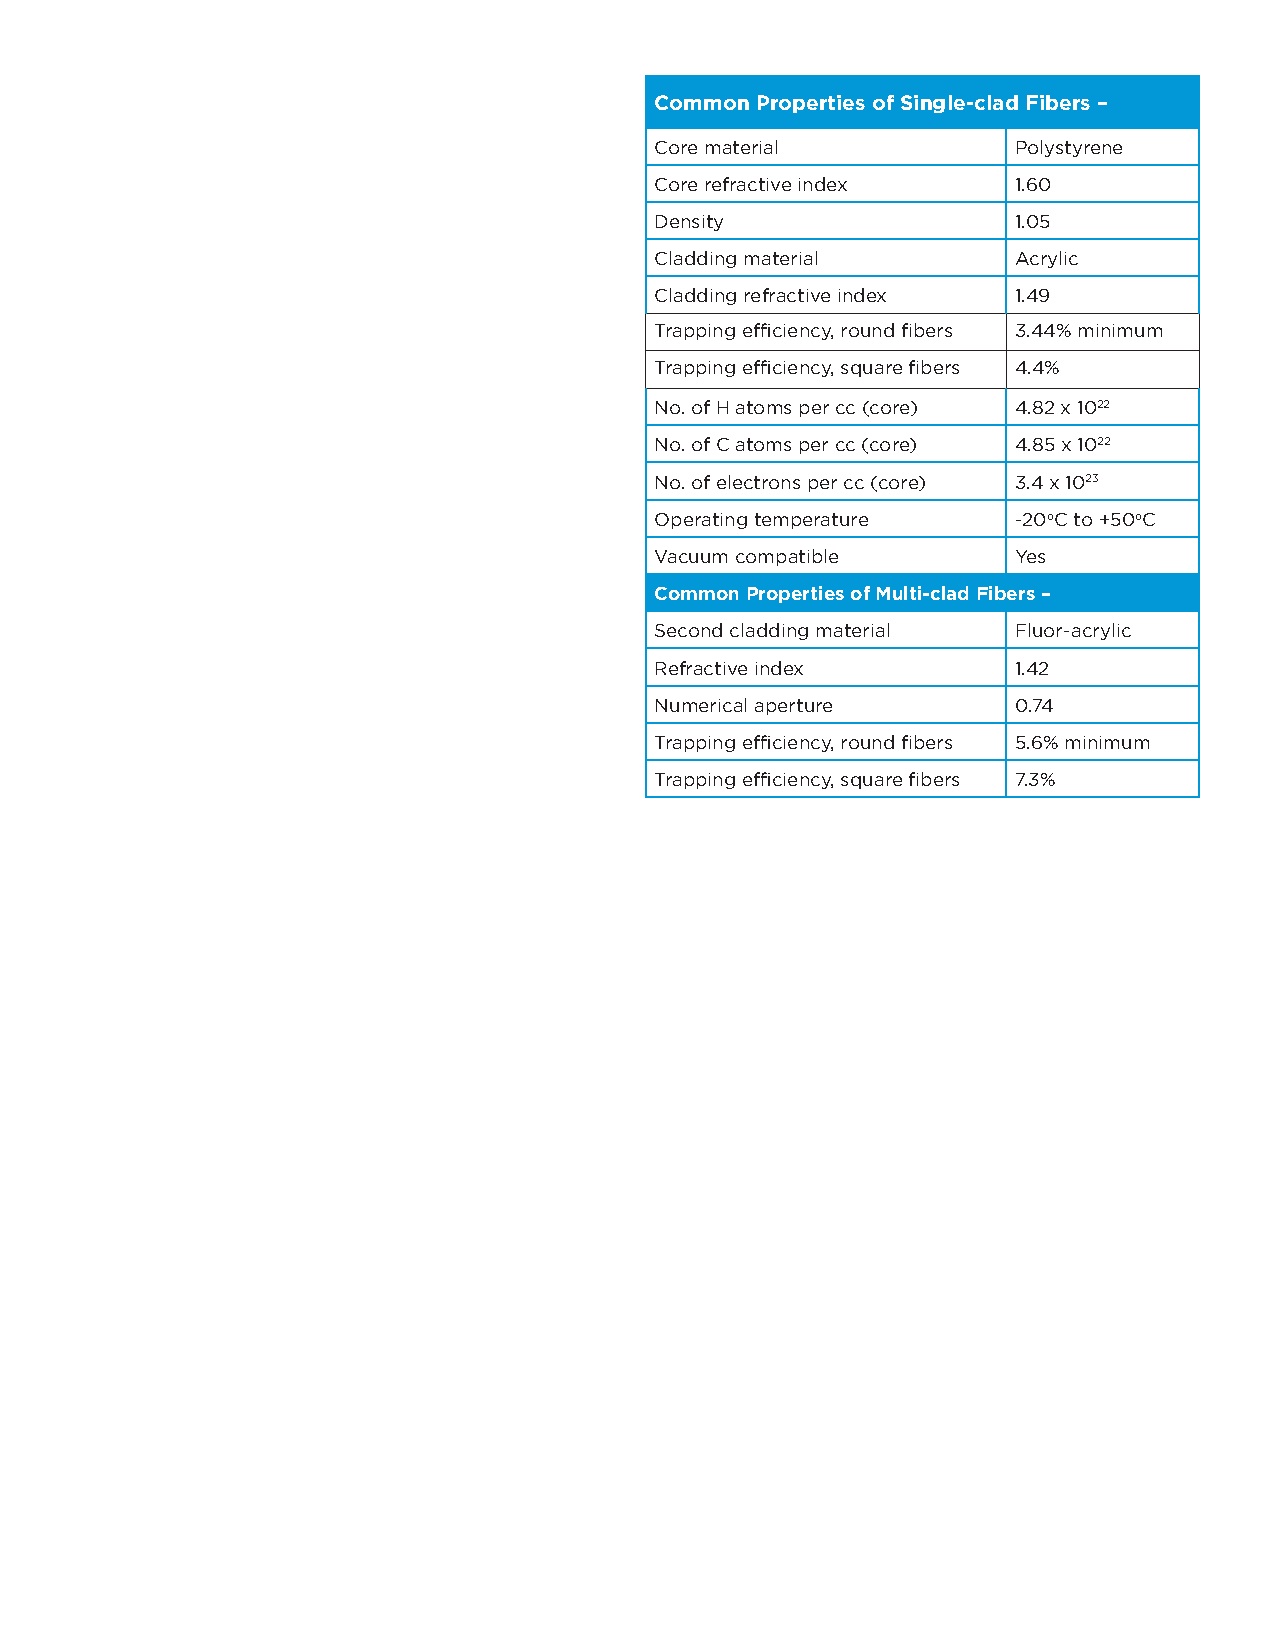
\includegraphics[scale=0.5]{img/fibersStGobain.pdf}
$\bullet$ Att. length for SG WLS fibres $>3.5$m.
  
 \column{0.5\textwidth}
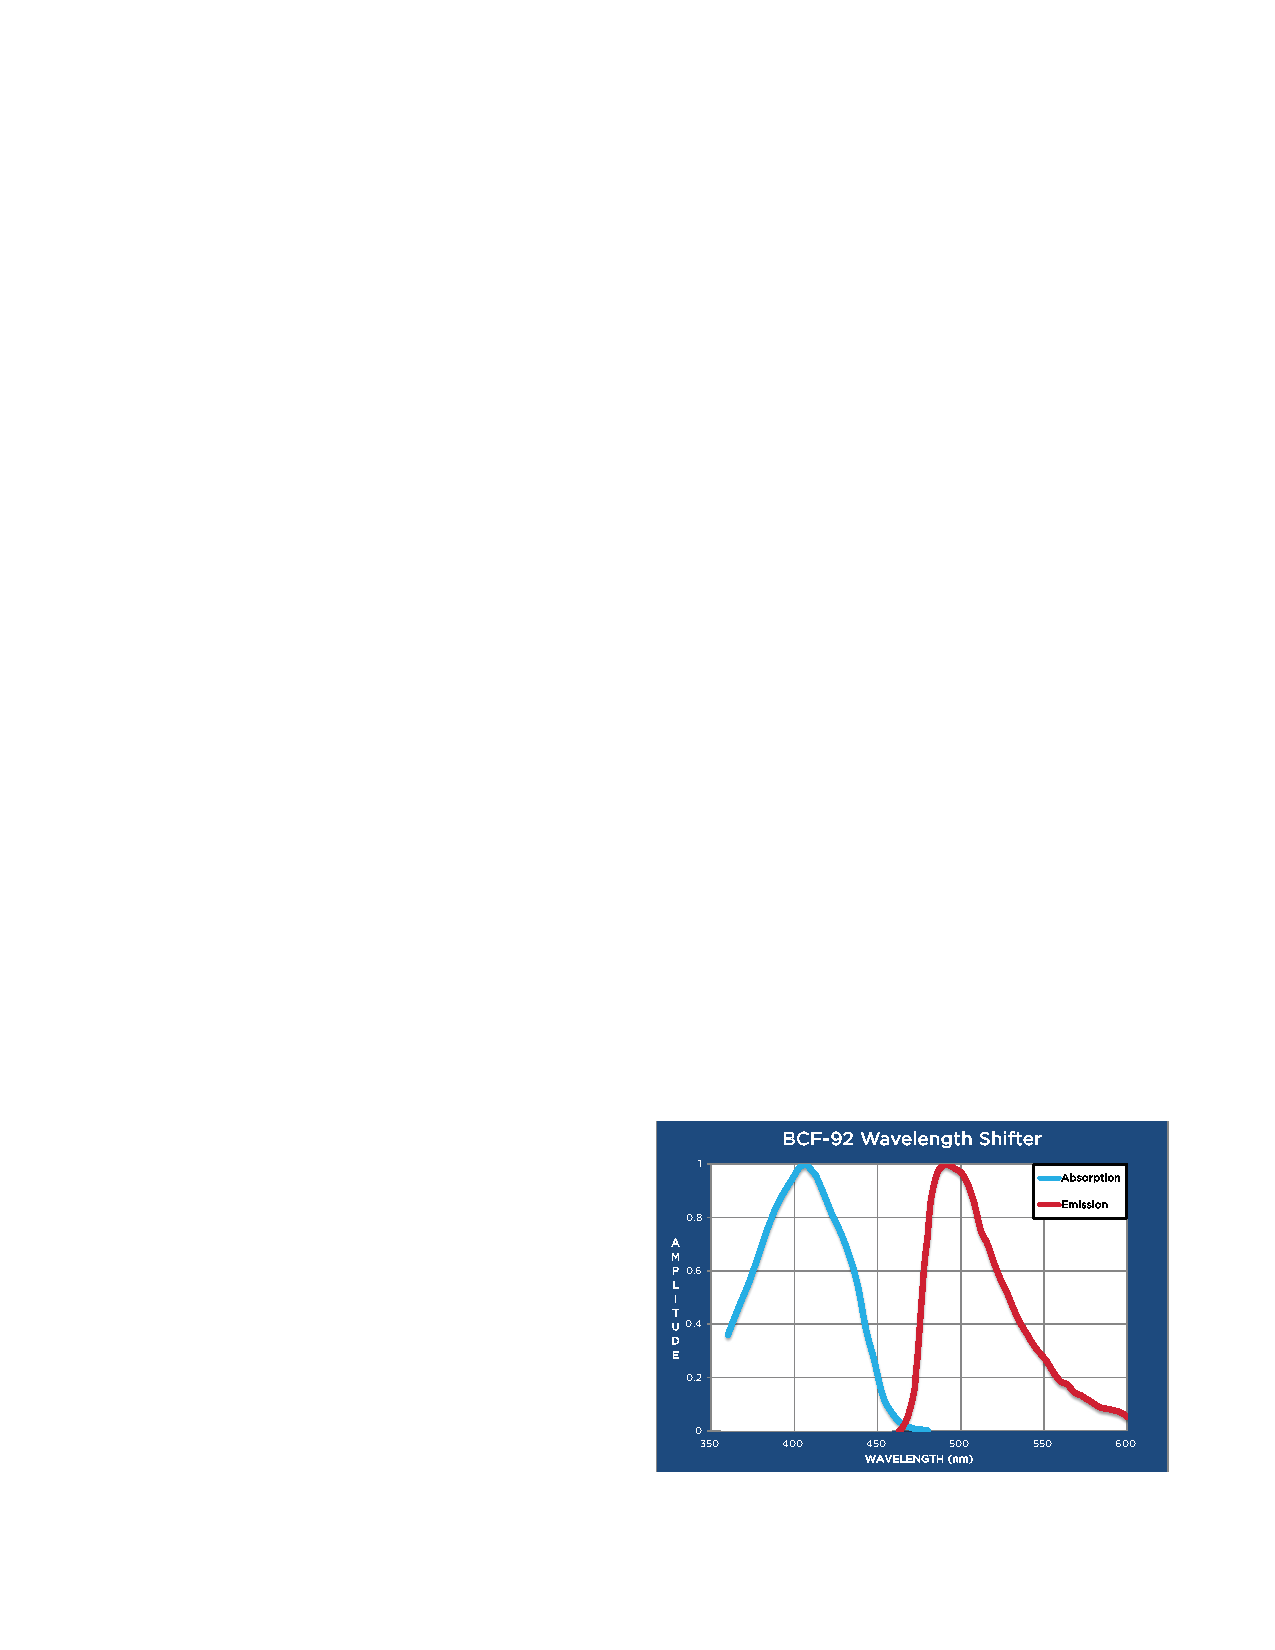
\includegraphics[scale=0.5]{img/wlsStGobain.pdf}

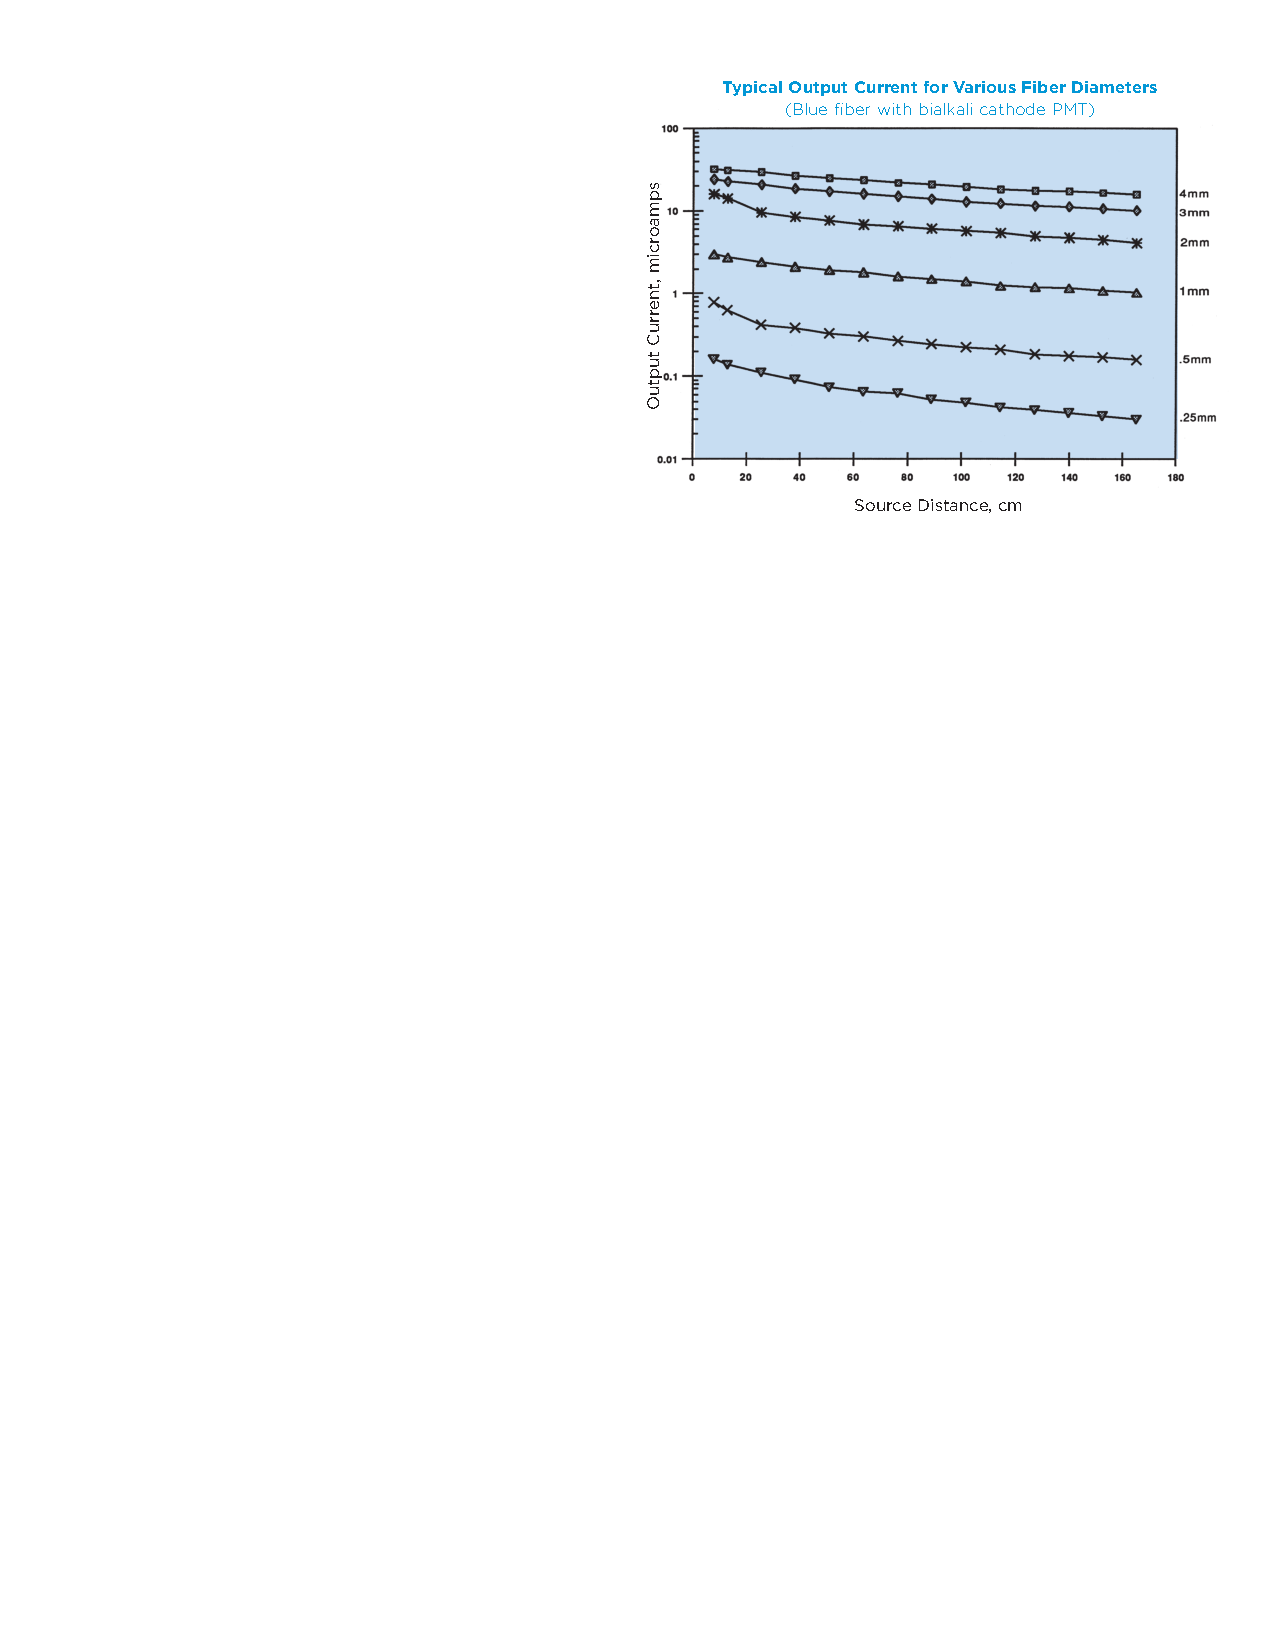
\includegraphics[scale=0.5]{img/fibAttLength.pdf}

\end{columns}
\end{frame}

\begin{frame}
\frametitle{Measuring \sone\ with fibers}


$\bullet$ The overall light collection efficiency of the BFD has been computed using full Monte Carlo simulation (JVM). A value of 3.0 \% is obtained assuming a QE  for TPB of 0.65 and squared fibres of \SI{2}{mm} size. Using previous values of QE for TPB (75\%) we find up to 3.5 \%. Finding a primary WLS with a QE $\sim$ 85\% would yield an efficiency of 4\%. 

$\bullet$ Adding one AFD will add an extra efficiency of 1.5 \% (QE $=$0.65) to
 2.0 \% (QE $=$0.85). Thus the combined efficiency of the BFD and AFD vary from
 4.5\% to 6\%. We will take 5\% as default value. 
\end{frame}

\begin{frame}
\frametitle{Reading fibres with SiPMs}
\begin{columns}
\column{0.45\textwidth}

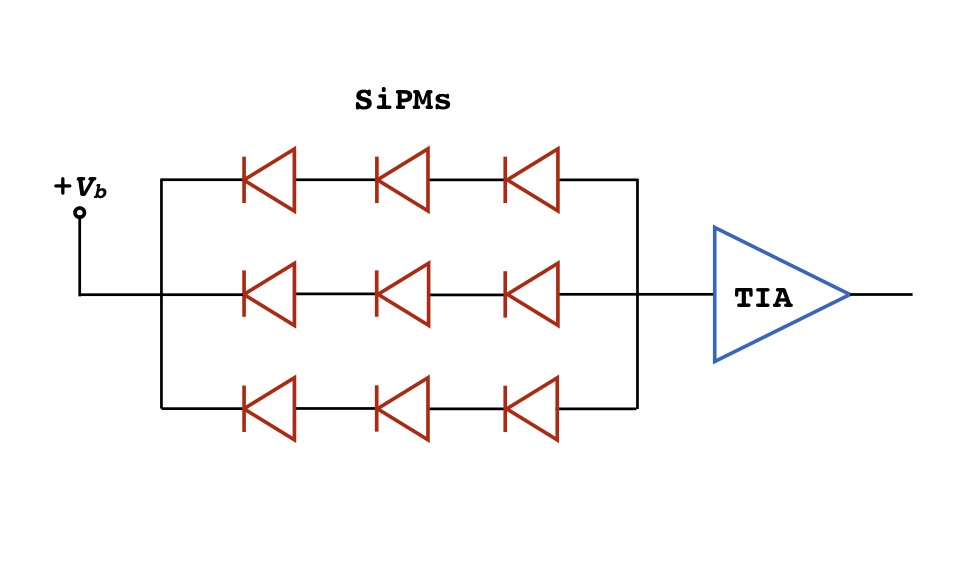
\includegraphics[scale=0.5]{img/3s3p.png}

$\bullet$ Each fibre can be read out with 4 SiPMs of \SI{1 x 1}{mm^2}, connected in a 2s2p scheme, similar to the 3s3p scheme used by Dark Side. This means that two pairs of SiPMs are connected in parallel and then the pairs connected in series. The overall effect is that the amplitude and capacitance of the system is the same than 1 SiPM of \SI{1 x 1}{mm^2}.
  
\column{0.45\textwidth}
 
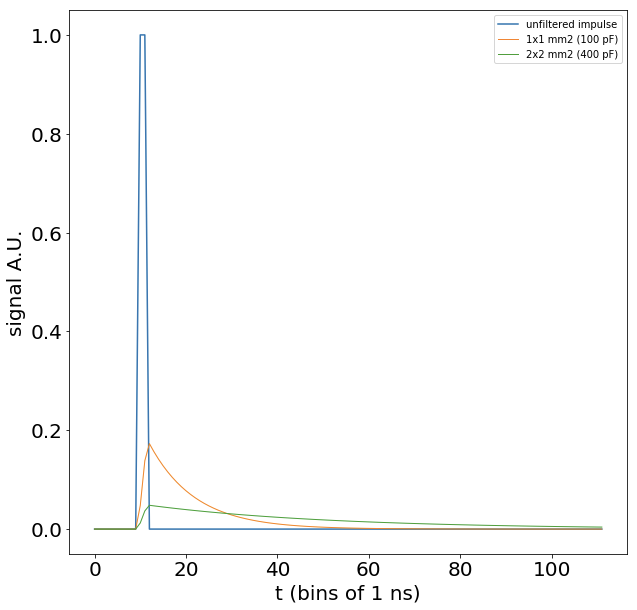
\includegraphics[scale=0.2]{img/sipmResponse2s2p.png}

$\bullet$ Given the relatively small capacitance of the 2s2p arrangement, the baseline is restored in \SI{50}{ns}. Sampling at 20 MHz is then possible to measure \sone\ in \SI{50}{ns}, integrating only the DCR corresponding to that interval. 

\end{columns}
\end{frame}

\begin{frame}
\frametitle{Signal and DCR for \sone}
\begin{columns}
\column{0.35\textwidth}


{\fontsize{6pt}{7.2}\selectfont 
\begin{table}
\begin{center}
\begin{tabular}{|l|l|}
\hline
\# fibers (2.0 mm) & \num{3.93e+03} \\
\# electronic channels  & \num{7.85e+03} \\
\#  SiPMs (\SI{1 x 1}{mm^2}) &  \num{3.14e+04} \\
Sc. phot. det. (Kr) &  \num{2.14e+01}\\
Sc. phot. det. (Qbb) &\num{1.27e+03} \\
Sc. phot. det.  per Fiber (Kr) & \num{5.45e-03} \\
Sc. phot. det. per Fiber (Qbb) & \num{3.23e-01} \\
 \hline
\end{tabular}
\end{center}
\end{table}%
}
\column{0.45\textwidth}
 
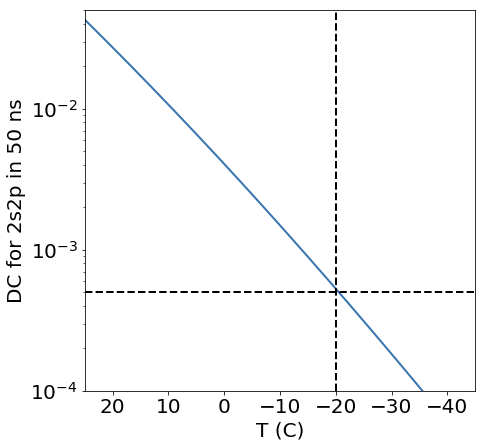
\includegraphics[scale=0.3]{img/dcrFibers2s2p.png}

\end{columns}
\blt {\bf Operating at \SI{-20}{\celsius} is possible to reduce DCR one order of magnitude below \sone\ signal at Kr (much better than that at \Qbb. Operation in the range \SIrange{-10}{-20}{\celsius} appears possible}. 
\end{frame}

\begin{frame}
\frametitle{Measuring \stwo}

\begin{table}
\begin{center}
\begin{tabular}{|l|l|}
\hline
EL phot. det. (Kr) &  \num{1.82e+04}\\
EL phot. det. (Qbb) &\num{1.08e+06} \\
EL phot. det.  per Fiber (Kr) & \num{4.63e+00} \\
EL phot. det. per Fiber (Qbb) & \num{2.74e+02} \\
 \hline
\end{tabular}
\end{center}
\end{table}

\blt\ No problems o dynamic range. Sampling at $\sim$\SI{2}{\micro\second} appears
straight forward. Photoelectron statistics is very large and does not affect the energy resolution. 
\end{frame}

\begin{frame}
\frametitle{A new concept for HD}

A possible design for HD would be:
\begin{enumerate}
\item A symmetric detector, of fiducial diameter \SI{250}{cm} and fiducial length \SI{250}{cm}, with drift length of \SI{125}{cm}.
\item Energy and \tz\ measured by a BFD and two AFDs. 
\item Tracking planes of similar design to those developed for \New\ and \Next. Small SiPMs (\SI{1 x 1}{mm^2}) at a pitch optimised for topology reconstruction (which in turn depends on diffusion, pitch and EL gap). 
\item Cool gas, with an operating temperature around \SI{-20}{\celsius}. Resolution expected to be OK at such temperature (LA measurements) and good gas stability. 
\item Investigate if electronics for tracking and energy can be the same (dynamic range). All electronics located behind copper shield. 
\end{enumerate}
\end{frame}

\begin{frame}
\frametitle{What about PMTs?}

\blt\ PMTs could be used to read out the WOLFs instead of SiPMs.  

\blt\ Fibres could be bundled to PMTs of suitable size (\eg \SI{50 x 50}{mm^2}), which could be held in individual pressure-resistant cans.

\blt The PMTs would be located behind the copper shielding, suppressing their radioactive budget. 

\blt\ This solution could minimise the number of channels and permit warm operation, but the challenges associated to coupling the fibres to PMTs, shielding and pressure-resistant vessels are significant.

\blt Furthermore, the lower QE of PMTs and possibly some losses associated to fibre bundling will result in significant less photoelectrons recorded for \sone. Thus, detection of Krypton may be difficult. 

\blt\ Alternative (pressure-resistant, radiopure) sensors, like the abalones could be another alternative (but still immature). 
\end{frame}

\begin{frame}
\begin{table}
\begin{center}
\begin{tabular}{|l|l|}
\hline
Scint phot, Kr, PMTs QE = 20 \%    & \num{8.12e+00} \\
Scint phot, \Qbb, PMTs QE = 20 \%  & \num{4.75e+02} \\
EL phot, Kr, PMTs QE = 20 \%   & \num{1.84e+04} \\
EL phot, \Qbb, PMTs QE = 20 \%   &  \num{4.25e+05} \\
 \hline
\end{tabular}
\end{center}
\end{table}%
\end{frame}
%\input{sipm.tex}
%\input{sipmBed.tex}

\end{document}